%%
%% Author: Moritz
%% 18.03.2018
%%

% Preamble
\documentclass[../../Pflichtenheft.tex]{subfiles}
\begin{document}
    \subsection{Rechnung}
    \begin{figure}[ht!]
        \begin{center}
            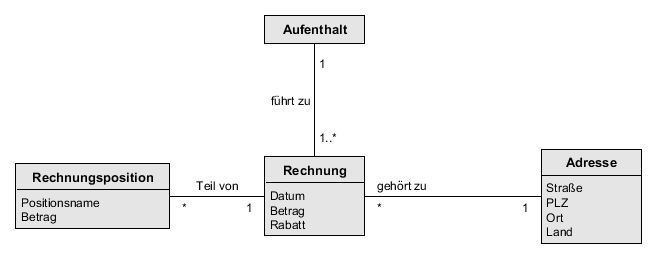
\includegraphics[width=0.5\linewidth]{assets/rechnung.png}
            \caption{Objekt 'Rechnung'} \label{rechnung_model}
        \end{center}
    \end{figure}
    Zu jedem Aufenthalt gehört eine Rechnung mit den entsprechenden Rechnungspositionen.
    Die Rechnungspositionen ergeben sich beispielsweise aus Extraleistungen oder Zusatzleistungen.
    Zudem ist jede Rechnung über den Aufenhalt inklusive der Reservierungsdetails mit einem Gast verknüpft und somit den Zahlungsdetails (nur
    im Gesamtmodell sichtbar). Zu jeder Rechnung gibt es zudem noch eine Rechnungadresse die nicht unbedingt
    der Adresse des Gastes entsprechen muss.
\end{document}